\documentclass[border=12pt]{standalone}
\usepackage{amsmath,amssymb,bm}
\usepackage{tikz}
\usetikzlibrary{positioning,arrows.meta,fit,backgrounds}
\tikzset{
  box/.style={draw, rounded corners=4pt, line width=0.8pt, inner sep=7pt, align=center, fill=white},
  stage/.style={draw, rounded corners=6pt, line width=0.8pt, inner sep=8pt},
  lab/.style={font=\bfseries\large, anchor=south west},
  arr/.style={-{Stealth[length=3mm]}, line width=1pt},
  darr/.style={-{Stealth[length=3mm]}, line width=0.8pt, dashed, gray},
}
\definecolor{cbulk}{HTML}{E3EEFB}\definecolor{cshear}{HTML}{E6F5E6}
\definecolor{ccent}{HTML}{FDF0E0}\definecolor{cchart}{HTML}{F3E6F7}\definecolor{cdata}{HTML}{F2F2F2}
\definecolor{cnote}{HTML}{FFFBE0}
\newcommand{\NN}{\mathcal{N}}
\newcommand{\re}{\operatorname{Re}}\newcommand{\im}{\operatorname{Im}}
\newcommand{\gb}{\bar g}\newcommand{\eb}{\bar e}\newcommand{\Eb}{\bar E}
\newcommand{\bnd}{\operatorname{b}}

\begin{document}
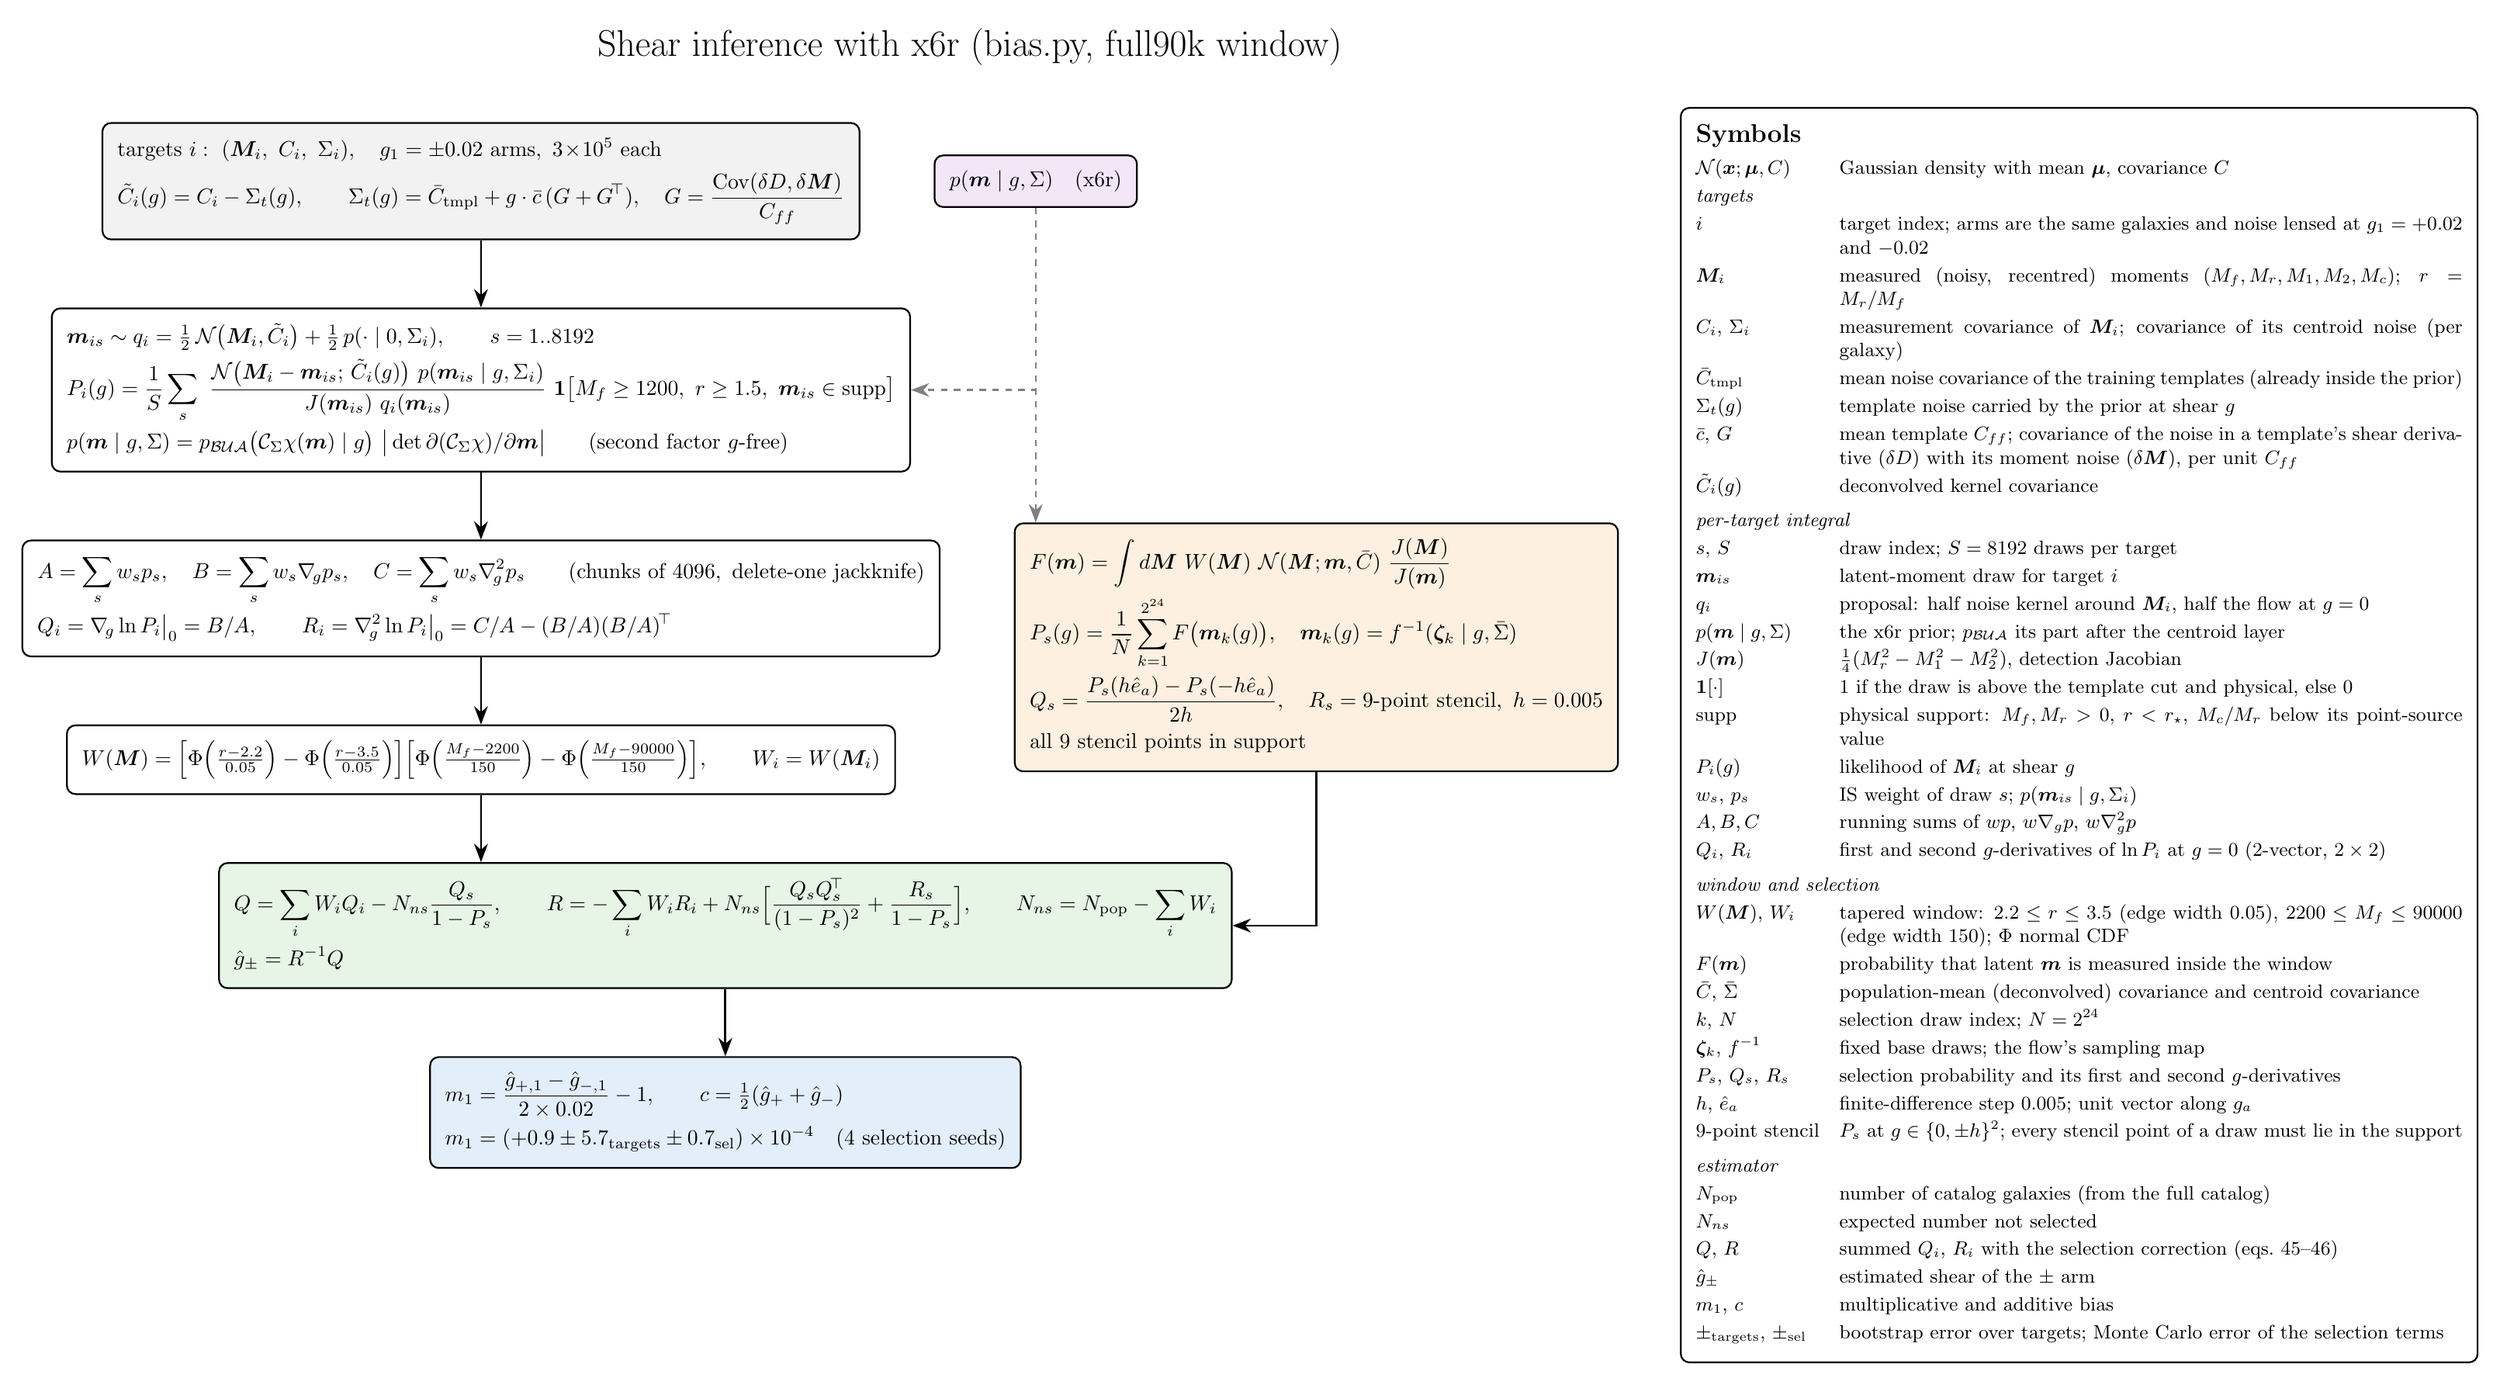
\begin{tikzpicture}[node distance=11mm]
\node[font=\LARGE] (title) {Shear inference with x6r (bias.py, full90k window)};

\node[box, fill=cdata, below=8mm of title, xshift=-80mm] (tg) {$\begin{aligned}
&\text{targets } i:\ (\bm M_i,\ C_i,\ \Sigma_i),\quad g_1=\pm0.02\ \text{arms},\ 3\!\times\!10^5\ \text{each}\\
&\tilde C_i(g)=C_i-\Sigma_t(g),\qquad \Sigma_t(g)=\bar C_{\text{tmpl}}+g\cdot\bar c\,(G+G^{\!\top}),\quad G=\frac{\operatorname{Cov}(\delta D,\delta\bm M)}{C_{ff}}
\end{aligned}$};
\node[box, fill=cchart, right=12mm of tg] (fl) {$p(\bm m\mid g,\Sigma)$\quad(x6r)};

\node[box, below=of tg] (is) {$\begin{aligned}
&\bm m_{is}\sim q_i=\tfrac12\,\NN\big(\bm M_i,\tilde C_i\big)+\tfrac12\,p(\cdot\mid0,\Sigma_i),\qquad s=1..8192\\
&P_i(g)=\frac1S\sum_s\ \frac{\NN\big(\bm M_i-\bm m_{is};\,\tilde C_i(g)\big)\ p(\bm m_{is}\mid g,\Sigma_i)}{J(\bm m_{is})\ q_i(\bm m_{is})}\ \mathbf 1\big[M_f\ge1200,\ r\ge1.5,\ \bm m_{is}\in\text{supp}\big]\\
&p(\bm m\mid g,\Sigma)=p_{\mathcal B\mathcal U\mathcal A}\big(\mathcal C_\Sigma\chi(\bm m)\mid g\big)\ \big|\det\partial(\mathcal C_\Sigma\chi)/\partial\bm m\big|\qquad(\text{second factor }g\text{-free})
\end{aligned}$};

\node[box, below=of is] (qr) {$\begin{aligned}
&A=\sum_s w_s p_s,\quad B=\sum_s w_s\nabla_{\!g}p_s,\quad C=\sum_s w_s\nabla^2_{\!g}p_s\qquad(\text{chunks of }4096,\ \text{delete-one jackknife})\\
&Q_i=\nabla_{\!g}\ln P_i\big|_{0}=B/A,\qquad R_i=\nabla^2_{\!g}\ln P_i\big|_{0}=C/A-(B/A)(B/A)^{\!\top}
\end{aligned}$};

\node[box, below=of qr] (win) {$\begin{aligned}
W(\bm M)=\Big[\Phi\Big(\tfrac{r-2.2}{0.05}\Big)-\Phi\Big(\tfrac{r-3.5}{0.05}\Big)\Big]\Big[\Phi\Big(\tfrac{M_f-2200}{150}\Big)-\Phi\Big(\tfrac{M_f-90000}{150}\Big)\Big],\qquad W_i=W(\bm M_i)
\end{aligned}$};

\node[box, fill=ccent, right=12mm of qr, yshift=-8mm] (sel) {$\begin{aligned}
&F(\bm m)=\int d\bm M\ W(\bm M)\ \NN(\bm M;\bm m,\bar C)\ \frac{J(\bm M)}{J(\bm m)}\\
&P_s(g)=\frac1N\sum_{k=1}^{2^{24}}F\big(\bm m_k(g)\big),\quad \bm m_k(g)=f^{-1}(\bm\zeta_k\mid g,\bar\Sigma)\\
&Q_s=\frac{P_s(h\hat e_a)-P_s(-h\hat e_a)}{2h},\quad R_s=\text{9-point stencil},\ h=0.005\\
&\text{all 9 stencil points in support}
\end{aligned}$};

\node[box, fill=cshear, below=of win, xshift=40mm] (est) {$\begin{aligned}
&Q=\sum_i W_iQ_i-N_{ns}\frac{Q_s}{1-P_s},\qquad
R=-\sum_i W_iR_i+N_{ns}\Big[\frac{Q_sQ_s^{\!\top}}{(1-P_s)^2}+\frac{R_s}{1-P_s}\Big],\qquad N_{ns}=N_{\text{pop}}-\sum_iW_i\\
&\hat g_\pm=R^{-1}Q
\end{aligned}$};

\node[box, fill=cbulk, below=of est] (res) {$\begin{aligned}
&m_1=\frac{\hat g_{+,1}-\hat g_{-,1}}{2\times0.02}-1,\qquad c=\tfrac12(\hat g_++\hat g_-)\\
&m_1=(+0.9\pm5.7_{\text{targets}}\pm0.7_{\text{sel}})\times10^{-4}\quad(\text{4 selection seeds})
\end{aligned}$};

\draw[arr] (tg) -- (is); \draw[arr] (is) -- (qr); \draw[arr] (qr) -- (win); \draw[arr] (win.south) -- (win.south |- est.north);
\draw[darr] (fl.south) -- (fl.south |- sel.north); \draw[darr] (fl.south) |- (is.east);
\draw[arr] (sel.south) |- (est.east);
\draw[arr] (est) -- (res);

\node[box, anchor=north west, align=left, font=\small, fill=white] at ([xshift=10mm,yshift=-14mm]current bounding box.north east) {%
\renewcommand{\arraystretch}{1.18}%
\begin{tabular}{@{}l@{\quad}p{10.2cm}@{}}
\multicolumn{2}{@{}l}{\large\textbf{Symbols}}\\[2pt]
$\NN(\bm x;\bm\mu,C)$ & Gaussian density with mean $\bm\mu$, covariance $C$\\
\multicolumn{2}{@{}l}{\textit{targets}}\\
$i$ & target index; arms are the same galaxies and noise lensed at $g_1=+0.02$ and $-0.02$\\
$\bm M_i$ & measured (noisy, recentred) moments $(M_f,M_r,M_1,M_2,M_c)$; $r=M_r/M_f$\\
$C_i$, $\Sigma_i$ & measurement covariance of $\bm M_i$; covariance of its centroid noise (per galaxy)\\
$\bar C_{\text{tmpl}}$ & mean noise covariance of the training templates (already inside the prior)\\
$\Sigma_t(g)$ & template noise carried by the prior at shear $g$\\
$\bar c$, $G$ & mean template $C_{ff}$; covariance of the noise in a template's shear derivative ($\delta D$) with its moment noise ($\delta\bm M$), per unit $C_{ff}$\\
$\tilde C_i(g)$ & deconvolved kernel covariance\\[3pt]
\multicolumn{2}{@{}l}{\textit{per-target integral}}\\
$s$, $S$ & draw index; $S=8192$ draws per target\\
$\bm m_{is}$ & latent-moment draw for target $i$\\
$q_i$ & proposal: half noise kernel around $\bm M_i$, half the flow at $g=0$\\
$p(\bm m\mid g,\Sigma)$ & the x6r prior; $p_{\mathcal B\mathcal U\mathcal A}$ its part after the centroid layer\\
$J(\bm m)$ & $\tfrac14(M_r^2-M_1^2-M_2^2)$, detection Jacobian\\
$\mathbf 1[\cdot]$ & 1 if the draw is above the template cut and physical, else 0\\
supp & physical support: $M_f,M_r>0$, $r<r_\star$, $M_c/M_r$ below its point-source value\\
$P_i(g)$ & likelihood of $\bm M_i$ at shear $g$\\
$w_s$, $p_s$ & IS weight of draw $s$; $p(\bm m_{is}\mid g,\Sigma_i)$\\
$A,B,C$ & running sums of $w p$, $w\nabla_g p$, $w\nabla_g^2p$\\
$Q_i$, $R_i$ & first and second $g$-derivatives of $\ln P_i$ at $g=0$ ($2$-vector, $2\times2$)\\[3pt]
\multicolumn{2}{@{}l}{\textit{window and selection}}\\
$W(\bm M)$, $W_i$ & tapered window: $2.2\le r\le3.5$ (edge width 0.05), $2200\le M_f\le90000$ (edge width 150); $\Phi$ normal CDF\\
$F(\bm m)$ & probability that latent $\bm m$ is measured inside the window\\
$\bar C$, $\bar\Sigma$ & population-mean (deconvolved) covariance and centroid covariance\\
$k$, $N$ & selection draw index; $N=2^{24}$\\
$\bm\zeta_k$, $f^{-1}$ & fixed base draws; the flow's sampling map\\
$P_s$, $Q_s$, $R_s$ & selection probability and its first and second $g$-derivatives\\
$h$, $\hat e_a$ & finite-difference step 0.005; unit vector along $g_a$\\
9-point stencil & $P_s$ at $g\in\{0,\pm h\}^2$; every stencil point of a draw must lie in the support\\[3pt]
\multicolumn{2}{@{}l}{\textit{estimator}}\\
$N_{\text{pop}}$ & number of catalog galaxies (from the full catalog)\\
$N_{ns}$ & expected number not selected\\
$Q$, $R$ & summed $Q_i$, $R_i$ with the selection correction (eqs.\ 45--46)\\
$\hat g_\pm$ & estimated shear of the $\pm$ arm\\
$m_1$, $c$ & multiplicative and additive bias\\
$\pm_{\text{targets}}$, $\pm_{\text{sel}}$ & bootstrap error over targets; Monte Carlo error of the selection terms\\
\end{tabular}};
\end{tikzpicture}
\end{document}
